\section{Biconditional Statements}

\begin{itemize}
    \item Recall that "$P$ iff $Q$ is equivalent to "If $P$ then $Q$ and if $Q$ then $P$".
    \item If you want to write a biconditional proof, write a proof for if $P$ then $Q$ and then write another proof for if $Q$ then $P$. 
\end{itemize}

\begin{proposition}
    The integer $n$ is odd if and only if $n^2$ is odd. 
\end{proposition}

\begin{proof}
    \subsubsection*{$\implies$}


    \subsubsection{$\implies$}

    Suppose $n$ is even. This means there is some integer $k$ such that $n = 2k$. This means that $n^2 = (2k)^2 = 4k^2 = 2(2k^2)$. Since $k$ is an integer, then $2k^2$ is also an integer. 
\end{proof}


\section{Equivalence Statements}

\begin{itemize}
    \item This is a generalization of biconditional statements
    \item We will use the phrase "the following are equivalent" (TFAE)
\end{itemize}

\begin{theorem}[The Invertible Matrix Theorem]{theorem6.1.1:def}
    WRITE THIS THEOREM HERE
\end{theorem}

    \begin{center}
        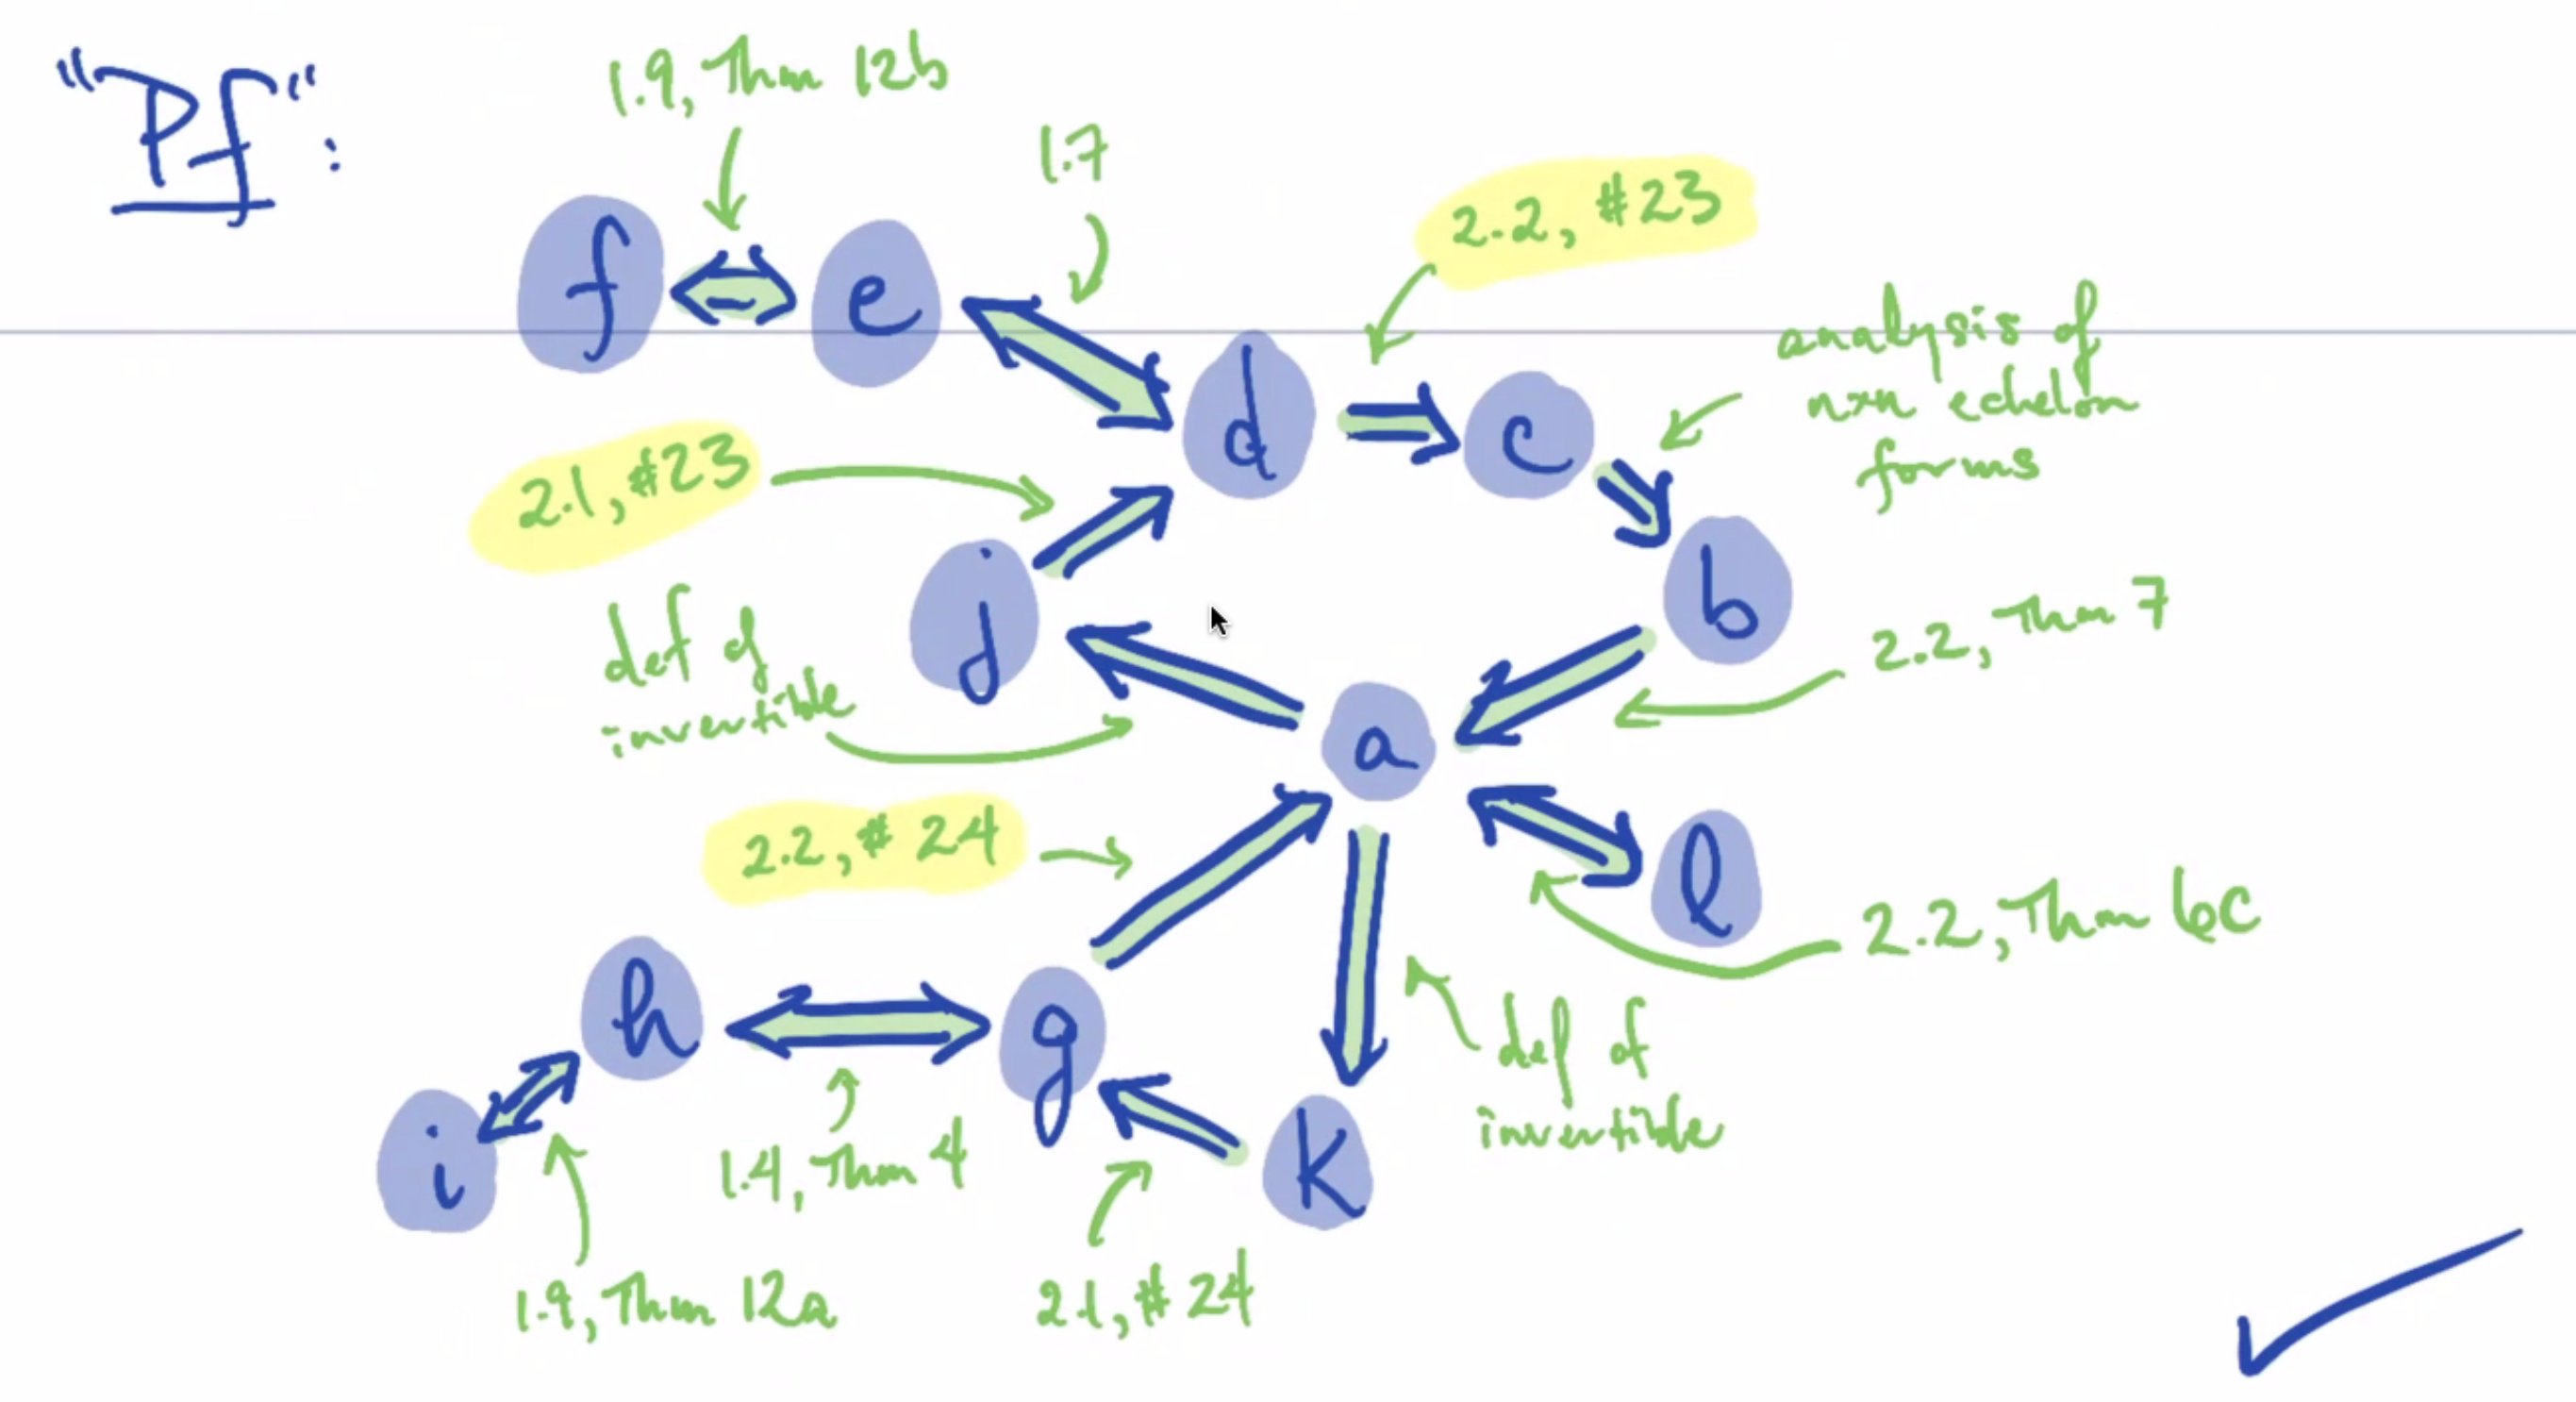
\includegraphics[width=1\textwidth]{chapters/ch6/images/fig6.1.PNG}
    \end{center}